% This example An LaTeX document showing how to use the l3proj class to
% write your report. Use pdflatex and bibtex to process the file, creating 
% a PDF file as output (there is no need to use dvips when using pdflatex).

% Modified 
\documentclass{l3proj}
\begin{document}

\title{MiniCooper}

\author{Gabor Mihucz \\
        Zay Yar Tun \\
        Pawel Heldt \\
        Nestoras Skiadas \\
        Corey Ansley}

\date{8 April 2019}

\maketitle

\begin{abstract}

This paper presents a case study of ``MiniCooper'', a project undertaken by a group of five Computing Science undergraduate students. In the paper, we will highlight our experiences using common software engineering methods and refer to a number of research papers outlining these methods.

\end{abstract}

%% Comment out this line if you do not wish to give consent for your
%% work to be distributed in electronic format.
\educationalconsent

\newpage

%==============================================================================
\clearpage
\setcounter{page}{1}
\section{Introduction}

The following document is a case study of ``MiniCooper'', an application software developed by Group 15 as part of Level 3 course on software engineering at the University of Glasgow. The main goal of the course is to deliver a tailored solution to a selected customer while working in a standard-sized agile team of five using professional software development practices.

Our group was required to develop a software tool for the Fife based software company ``Cooper Software'', represented by  Darryl Rankin, Head of Development. Our product, with the working title ``MiniCooper'', was intended to be a combination of a web and desktop application, which would upload local employees’ PDF files onto a server, processing them so that the most important information is extracted and stored in a user-readable JSON format.

Apart from developing a workable product, part of our assignment was to try various techniques and processes which are commonly used by professional development teams. These were mostly covered on ``Professional Software Development'', a Level 3 course by Dr Timothy Storer. This requirement distinguished our project from any other that we have conducted so far, as it made us pay a great attention not just to the quality of our code but to our professionalism as well.

In order to meet the set expectations, we have tried to empirically evaluate the effectiveness of multiple software development techniques and processes such as Scrum, Kanban, version control, continuous development/integration, pair programming and code reviews which were introduced to us before and over the course of the project. 

The delivery of the product was distributed into six ``iterations'' with each having time frames of four to eight weeks. At the end of each iteration, we were expected to deliver and demonstrate an agreed set of features we developed during the iteration to the customer, gather feedback and then discuss requirements for the next iteration including the priority of each new feature.

This document is structured in order to best represent the workflow of our team, with the first sections disclosing initial requirements and motives behind the application as well as design decisions. After that we describe the progress the team has made throughout the six iterations. The dissertation ends with a conclusion which reflects on the final outcome and the experience we gained thanks to working in a professional software development environment.
%==============================================================================
\section{Case Study Background}
\subsection{Customer and Objective}

Cooper Software is a software development company founded in 2005, based in Fife, specialised in Enterprise Resource Planning (ERP).

The company itself has to deal with great communication overhead such as hundreds of PDFs over the course of a week. The PDFs can be classified into a number of distinct groups based on their structure and titles: flight tickets, supermarket bills, etc. The relevant information happens to be at the same area in each PDF that belongs to a specific group. The company needs to retrieve this data and store it in an online system. Currently, there is an employee in the company who has to take time out of their regular work to manually open these PDFs and type the data into an online form, e.g. on a supermarket bill the labels to be entered manually could be: invoice number, address, total, etc.

Our task was to automate this process by creating an application that would automatically upload PDFs appearing in a specific folder, match the PDFs based on patterns in their filenames to custom templates the user created previously, convert the files to JSON using OCR (Optical Character Recognition) and display the data in a user-friendly interface.
Implementing a piece of software which would tackle this problem would result in less error-prone bookkeeping as user error is inevitable when it comes to typing. Furthermore, the employees could spend their time at work doing more creative or complicated tasks which is an additional business value for the company.
%==============================================================================
\subsection{Final Product Features}

One of the main features of the application is the highlighting areas on PDF defined by a template. To achieve this, we created a tool to \textbf{create and define templates for the PDF files to be matched to}. This is a canvas tool that uses two javascript libraries (Paper.js and PDF.js) where users have to upload a PDF as a background, highlight areas of interest and name those areas. After this task is completed the user can save the template and complete the configuration in a template manager.

\textbf{Template Manager} is a page where users are able to control previously created templates. This includes setting file patterns the template should look out for when new PDFs are uploaded, deleting selected templates and finally editing the template itself. Deleting the template will also delete previously created PDF conversions where this template was applied.

The program \textbf{filewatcher.py} runs on the employee machine and is based solely on Python. Its purpose is to upload all of the PDF documents which appear in a designated folder onto the web server.

The \textbf{web server and web application} are built with Django, a Python-based web development framework. The benefits of Django were that the whole team had significant experience with it already, it provides a built-in Admin page and user authentication and it is a straightforward, easy-to-use implementation of the MVC framework with plenty of documentation and a helpful community.

An uploaded PDF is processed by storing it in a database model that contains the file itself, the file name and the date when the uploading occurred. While the PDF is being uploaded \textbf{the system examines whether the filename matches any of the patterns associated with the user-created templates}. If a matching template is found the PDF is converted to .jpg with pdf2image. Then the image is cropped according to the coordinates of the template using numpy. Finally, \textbf{the cropped images are processed with pytesseract, an optical character recognition library} which uses pre-trained neural networks to recognize text in an image. The resulting JSON file which consists of the template keys linked to the extracted text is stored in a database model instance.

\textbf{On the main page, we display the links to PDF and JSON files}, the template’s name that was used during conversion and the upload date. The PDF and JSON files can be opened by clicking on them: the JSON data is rendered to a user-friendly representation of the key-value pairs.

The data is automatically loaded via an AJAX call, and the table is paginated with sorting and searching implemented with the DataTables jQuery plugin.

\textbf{There are two types of users}, regular users who can see the main page with converted files, and administrators who can create and edit templates as well as manage other users on the Admin page.



%==============================================================================

\subsection{Design Decisions}

The final product is based on the Client-Server architectural pattern, specified by the architecture diagramme presented below:

\begin{figure}[h]
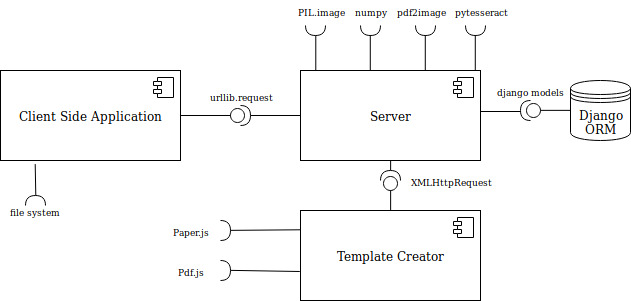
\includegraphics[width=0.7\textwidth]{figures/ComponentDiagram.png}
\centering
\caption{Component diagram of the application}
\label{fig:componentDiagram}
\end{figure}

As the software is intended to be used locally by a small- to medium-sized group of users, it is beneficial to implement its server in a centralised manner. The benefit coming from such a design is the improvement in the management and organisation of data, as all of it can be maintained and controlled in a single and consistent structure. Hence any future improvements can be undertaken directly on the server rather than simultaneously updating multiple clients. \cite{YadavSingh}


%==============================================================================
\section{Reflections}
\subsection{Iteration One and Two}

We spent Iteration One with getting set up and getting to know each other better to identify each others’ strengths  in order to assign technical tasks efficiently in the future.

We set up our GitLab account, installed the virtual machine we had been provided on the lab machines and familiarised ourselves with Linux. We also created a Slack account in order to communicate efficiently in the future on multiple channels and participated on a 48-hour Hackathon, partly as a team building exercise. Social Media would also be used for brief, and urgent, messages.

Iteration Two started with the team being assigned to our customer, Cooper Software. The goal for the end of this iteration was to have a detailed backlog, consisting of the detailed description of the project, and a clear well-organised set of tasks in GitLab to start delivering features.

The first step was to gather requirements, for which we needed frequent contact with our customer. Since he was based 70 miles away, we decided that the best way to keep in touch would be on Slack with occasional video conferences.

As expected in the initial requirements gathering phase, features and requirements were added, removed and changed on an ongoing basis. Requirements gathering was an iterative process, in which the team gradually increased clarity about the required features and its priorities.

In order to foster the creation of a common understanding of the requirements, we decided to create various forms of documentation in order to ensure that we were on the same page with the customer. We created:
\begin{itemize}
\item User Personas who represent the primary types of users who would interact with the app we would build.
\item An initial architecture diagram which would explain the general information flow of the application.
\item Wireframes, using a method our coach suggested: 
Each member of the team drafted five possible wireframes for the main page of the app, then explained their ideas to the rest of the team. After that, each member of the team drafted two suggested wireframes and explained his decisions to the rest of the team.
Finally everybody was required to draft one wireframe, and to everyone’s relief the proposed wireframes converged significantly.
\item User stories for the main features of the app. As per the request of our customer, we aimed to have user stories written from a non-technical end user perspective. Each user story was designed to be as atomic as possible, with the terse structure of ``As a [type of user], I want to [action  describing  feature], So that [action  describing  benefit  of  feature]'' \cite{CohnMike}
\item A very helpful technique we employed here was the Value Proposition Canvas, which helped us empathise with the customer, identify the core business value the application was creating, and the issues it was meant to resolve. This knowledge helped us tailor our solutions to the customer’s needs.
\end{itemize}

As suggested in the Principles behind the Agile Manifesto \cite{agilewebsite} , we welcomed changing requirements.
The final documentation is the result of many iterations of the following process:
\begin{itemize}
\item Creating documentation artifacts
\item Discussing the documentation artifacts with the customer
\item Taking notes of new or changed requirements
\end{itemize}

Following that, we used the MoSCoW method \cite{CleggBarker} to identify the most important features to implement in the coming iteration as ``Must-Haves''. These were: 
\begin{itemize}
\item Basic web app
\item Create predefined template
\item Prototype for file conversion from PDF to JSON via predefined template
\end{itemize}

We uploaded all the gathered requirements and produced documentation to the Wiki page of GitLab.  Initially, we uploaded the list of user stories to the wiki as well, and we added technical tasks to be done to deliver features to the board with labeled due dates.

We started to diversify our communication to multiple channels on Slack to reflect the growing complexity of the project: we prepared for the coming meeting with the customer on the channel \#presentation, while we created a very handy channel \#guides, where we copied useful commands and reference guides, e.g. how to log in to the Virtual Machine (which we planned to use for CI/CD purposes), how to install a virtual environment and dependencies, recurrent git commands, etc.

Since occasions to meet the customer in person were scarce, we tried to maximise the benefits of the customer meeting by having a well-structured presentation of our accomplishments thus far and our planned deliverables for the coming iteration. We planned the meeting so that each team member would get to talk about their share of tasks in the first half of the meeting and we would have time for an open discussion with the customer in the second half. However the customer preferred to have a dialogue-like meeting throughout, which made us to improvise on the spot. The meeting overall went very well, but having learnt from the experience of the first customer meeting, we decided that in following meetings we would share the responsibilities differently: one team member would present the slides, two team members would respond to the customer’s questions and ask for clarifications/more details in case of new requirements, and two team member would act as observers/note takers. Once the main customer meeting was done, we discussed the notes taken during the meeting so that everyone was on the same page, with clear tasks for the next iteration. The final notes would also be shared with the customer later on to verify that the requirements, as we understood, were indeed what he wanted. This would be repeated after every customer meeting.

After the customer meeting, we also had our first retrospective. Retrospectives are crucial for a modern software development process; they force the developers to look at the bigger picture, ironing out the methods and practices employed by the team so that productivity and efficiency is maximized. They give team members a chance to vocalise any grievances they might have had during the development process in the appropriate time and environment. Airing grievances at an inappropriate time can make a developer feel insecure, whereas proper retrospective meetings allow for a healthier environment for criticism and self improvements. \cite{DerbyLarsenSchwaber} 

Frameworks are a great help with structuring retrospectives. A retrospective framework describes a technique by which all team members offer their criticism in organised manner that allows the complaints to be grouped according to categories by the end of the meeting. For this specific retrospective, we employed the ``Liked-Learned-Lacked-Longed For'' framework. One of the ways that a retrospective allows for a healthy environment is by including positive remarks that balance out the negativity of the complaints. Remarks by the team are written under the four columns, which scale according to importance from left to right. Ideally, the team will learn some useful lessons from the retrospective and successfully hone their teamwork skills. In hindsight, we conclude that our first retrospective had vague suggestions and criticisms, and we did not identify solutions to the issues raised.

%==============================================================================
\subsection{Iteration Three}

One of the greatest sources of ambiguity in the requirements for our project was how the functionality of the project was going to be split between the local application and the web-based one. Some of this division was clear; the file watching feature was going to be on the local application and the template creator was going to be on the web application. For other features, such as the Optical Character Recognition and the viewing of the results, the team was instructed to develop this on the side of the web application.

As our customer is a software engineering firm, their representative was able to give us some feedback on our software engineering practices and more specifically on our issue tracking methodology. We were advised to minimise the duplication of tasks on our virtual KanBan board \cite{Skarin} and to organise our technical tasks under the non-technical user stories using dependencies, which we adhered to until the end of the project. User stories and technical tasks were distinguished using labels, and each issue was assigned to a specific iteration. KanBan boards can be an important part of an Agile developer’s toolbox, since they allow for issues to be categorised by their state in the development pipeline in an easy to read manner.

Organising the KanBan board like this allowed us to easily filter it by:
\begin{itemize}
\item High level user stories only (important for the customer)
\item Technical tasks
\item Issues assigned to a specific team member
\item Other labels such as ``high priority'' or ``QA'' (Quality Assurance)
\end{itemize}

In many ways, Iteration 3 constituted the point at which we began development of the application in earnest. For a simple overview of the features delivered in this iteration, we created a ``Hello World'' application in the Django web-app framework, implemented user authentication functionality and fleshed out a significant part of the User Interface. On the local application side, we created a hard-coded template that was used in conjunction with OCR to process some premade PDF files.

To start with, we created a small script that would crop an image according to two pairs of coordinates which formed a rectangle. Then, we initialized a Django project, which would allow us to develop the web application further down the line. Another small script was created - this one was exploratory in nature, as we were learning how to utilize the tesseract library. Importantly, this piece of code was accompanied by our first unit test. Throughout development, we made sure to create unit tests as we were developing features. This habit helped us maintain a high coverage percentage throughout the development process.

During the end of the iteration, we had a customer demo. Since the team had only started on the development of the app and did not have much to show for the demo, we decided to use prototypes and wireframes as substitute. It was found to be effective as instead of trying to explain the future features using words, a picture (with some narration) displays more information and the customer was easily able to catch onto what we were planning to deliver and give us almost immediate feedback. As such, we also decided to use wireframe/prototypes in future demonstrations.


%==============================================================================
\subsection{Iteration Four}

This iteration spans across two months including the winter holidar so we decided to split it between two shorter sprints. 

Before the end of the semester, the team had assigned clear tasks to each other which were also tracked in the issue board. We also started using planning poker \cite{MikeAgile} , and added the estimated delivery efforts as numbers next to each issue. This organisation helped us stay motivated during this period. 

During the middle of the break, there was a disruption to the university network which rendered us unable to access the repository as well as the issue tracking system which hindered the progress of the team. Not only we were unable to access the latest file or update the repository, we were also not able to track issues which is necessary for task delegation until the break was over. We decided to move to a temporary repository on the public Gitlab and later migrating back to the university Gitlab. The commits pushed during the server downtime are only accessible in the temporary GitLab repository.

The other main tasks for the web app in the iteration were:
\begin{itemize}
\item To develop and improve the back end
\item Moving our cropping and processing code we had written in the local application into the web application for multi-platform compatibility.
\item Setting up a user system as in the design of the project by having regular users and admins
\item Development for the main result page
\end{itemize}

A few missed objectives include user friendly representation of JSON data on the main page, error checking when PDF is converted into JSON. The first was missed due to us not assigning the right person for the task and the second being due tests not being written for the fix on time and as such, the update was not pushed on time for the iteration.

As the team got more used to the Gitlab system, we developed and improved the continuous integration pipeline and as requested by the customer, the pipeline was to be designed to also produce an artifact that would allow the customer to be able to deploy the latest build of the software. In order to ensure user friendliness, a user guide was required that would make it easier for the customer to deploy. The pipeline would try to build the software from scratch every time a commit was made, this is necessary to make sure that every time a change has been made, the software would not break when being installed on a new system.

The team also decided to step up on the quality assurance department and one of the goals in the iteration was to achieve high test coverage across the files by filling it up with meaningful tests. Having a high-test coverage would reduce defects as almost every single part of the code would be tested every time the test suite was activated, which occurs with every commits to the repository as it is attached to the continuous integration pipeline. This means that every time an update was made to the codebase and parts were changed, we can ensure that it does not break other parts of the code and this reduces the risk overall.

The iteration ended with another successful demonstration to the customer, followed by a retrospective. During the retrospective, the team used starfish technique following the suggestion of the team coach. This retrospective contains five different sections, namely: Start, Stop, Continue, More of and Less of \cite{GoncalvesLinders}. The team agreed to:

\begin{itemize}
\item Start doing dissertation studies and communicate via issues
\item Stop pushing too late before the meeting and stop being late to the meetings
\item Less of being distracted in meetings
\item More of testings, code reviews, comments, motivation, making sure VM works
\item Keep doing great demos, good communication and task delegation
\end{itemize}

One realization we had after the retrospective was that we were not keeping clear track of how well we are implementing the solutions the team agreed to have after the previous retrospective. For example, to avoid becoming distracted, a constructive solution was to try to implement the pomodoro method. \cite{Cirillo} The team decided to utilize the issue board, creating a different type of issue labelled as “Retrospective Solutions” on the issue board, moving them between stages similarly to any other issues on subsequent meetings, as we assessed ourselves how good we are at sticking to the identified solutions. Overall, the team managed to accomplish most of the tasks set for the iteration and was able to follow up on most of the retrospective solutions despite a few hiccups.


%==============================================================================
\subsection{Iteration Five}

In this iteration we wanted to finish all the main features of ``MiniCooper''. We could then leave bug fixes, polishing and perhaps some minor features for Iteration Six and be ready to deliver.

We wanted to have our app deployed on one of the customer’s machine, following the Agile principle of delivering working software as often as possible. \cite{agilewebsite} Our customer had been happy with our progress so far but we knew we could get more valuable feedback from leaving it in his hands.  

This iteration we began user testing as we wanted to get feedback from outside the development team that we could not get from our customer until he deployed the software. We asked people unfamiliar with the project, preferably not computing science/software engineering students, to try our application and give us feedback on the usability of the app. We created a google form for them to provide their feedback. The main benefit of user testing was however, the bugs that were discovered. We realised that we were not going to get valuable feedback on the app until we address these, hence each bug was entered to GitLab with high priority, and solved as soon as possible.
We were glad that user testing helped our software become more robuts, however, possibly we could have used testers time on more valuable work such as feedback on UX, if we had implemented more thorough testing before.

During both this iteration and iteration 6 we increased the number of code reviews we did in order to prepare for delivery. During these code reviews we identified a number of ``bad smells'' \cite{Fowler}. A example of this was in the template editor and template creator where we found significant amount code duplicated across the two files. We decided to refactor in order to follow the principle of Don’t Repeat Yourself (DRY) \cite{HuntThomas}. We extracted functions from the code and replaced any occurrences of the duplicate code with calls to one of these functions. Refactoring is an important task in software development as it lowers the cost of developing new features in the future as well as making the codebase much more understandable. This not only improves the quality of the code but also reduces the risk of code breaking down.

Overall the iteration was a success; all critical features were finished however, we did have some missed objectives. Despite our frequent communication via Slack and email, our customer did not find the time to deploy the app to provide us with a feedback. Two lower priority objectives were: the ability to resize boxes by their corners in the template creator and the automatically refreshing result page. Box resizing turned out to be too demanding of a task with the library of our choice. Automatic refreshing of the index page was implemented however, the newly implemented functionality collided with the previously implemented pagination and we could not find a workable solution at that point. After discussion with our customer it was decided that pagination was more important than the refreshing but both working together was still desired. Therefore we rolled back this code for now so that pagination still worked and left automatic refreshing as a missed objective. 

By the end of this iteration, we got used to doing retrospectives, and every team member had multiple solutions to each identified issue. The more concrete solutions we came up with at the last iteration had been a great success in improving our productivity, we met most of our goals and made significant progress. This is why we once again used the starfish technique for this retrospective and identified  even more concrete solutions. Some examples included assigning regularly a task to update our wiki or committing ourselves to one code review each week. Another identified issue was the constructive criticism which was not efficient enough throughout the meetings and decreasing interaction on Slack. The proposed solutions were: set agendas for meetings, and that each team member should react with at least an emoji to each Slack post.
In order to stay on track with all the issues that need to be closed, we decided to start setting deadlines for tasks, and we agreed that if someone misses a deadline, then the reason behind it should be explained before granting an extension.

%==============================================================================
\subsection{Iteration Six}

One of our biggest priority in this iteration was Quality Assurance. We wanted to make sure the final version of ``MiniCooper'' was easy to use and free of any critical bugs.

From the very beginning we had focused on testing.  We increased the volume of tests as much as we could as well increased test coverage across the entire server side of the application. We had wanted to also include testing of our javascript files, however in the end we didn’t have to time implement these due to the team not prioritizing it soon enough and the team did not manage to get it working on time.


Probably the biggest challenge this iteration was assisting our customer to deploy our app. A final requirement change meant that the web server had to be able to be run on Windows as well, not just on Linux. A Windows install script and user guide had to be written quickly and Windows deployment introduced new bugs even though Python is meant to be platform-agnostic. For example, we noticed that the website would not display non-ASCII characters correctly. It was so because of the difference in UTF encoding, which turned out to be a bug hideous but trivial to repair. Discovering it underlined the importance to test the application on both operating systems.

We managed to complete the Windows deployment within a few weeks before the deadline, however, we had not heard back from customer about his experience with it. 

By the end of this iteration we were confident that we were ready to deliver our application. All the main requirements had been added, though we were still missing some optional features. We had also managed to re-implement automatic refreshing with pagination on the results page switching to using DataTables.

We did not have a retrospective by the end of this iteration, but we evaluated our previous retrospective solutions. We agreed that they further improved our communication and overall performance leaving us with a functional working environment by the end of the project.

%==============================================================================
\section{Conclusions}

In hindsight, the conclusions we can draw can be enumerated as follows:

\subsection{Initial Requirements Gathering and Planning Phase}

Requirements are quite vague in the beginning, as the project takes shape. Project documentation, such as user personas, wireframes, site URLs, UML diagrams take time, but help immensely to create clarity between the development team and the customer.
Once the initial requirements are agreed, it is a good idea to produce a quick prototype. This gives the customer the opportunity to further clarify requirements, and the team to quickly change and adopt to these. Following a successful prototype and agreed requirements, it is useful to identify the scope of the project and decide on web frameworks to use. Django was an excellent choice for the backend, however we would have benefited from a front-end framework such as React or Angular for multiple reasons: automated testing would then have been very easy to implement and we could have enjoyed better library and community support.


\subsection{Project Management and Development}

As it was expected, Team Dynamics evolved throughout the course of the project: as we got to know each other better, and got used to working together, we could better estimate the delivery costs of certain features and our understanding of the frameworks and tools we used increased. We found retrospectives the best tools to improve our team work, especially when we decided to suggest concrete solutions to the identified issues and adhered to them improved the team's commitment and efficiency in the project. 


\subsection{Quality Assurance}

Although the backend is thoroughly tested with over 90\% coverage, our front-end lacks tests. This is partly due to not using any front-end frameworks, partly to occasionally prioritising delivering features over thorough tests.
We started user-testing late, which revealed several bugs at the end of the project. Due to the complexity and unusual nature of the app (as it is meant to be used in a company setting, not by individual users), user testing was difficult to organise and get useful results. Each user test would first need a thorough brief and setup, which is fairly time-consuming and resource-intensive. An alternative option could have been to gather 10-15 users into one physical place, brief them and make them test the app at once in order to save time and introduce competition among them to think of unusual edge cases to be tested.


\subsection{Final Notes}

Since the start of our degrees, the Team Project was possibly our biggest step up in our journey to become professional software developers. This was the first time we worked in a reasonably large group for an extended amount of time creating software for a real world customer. Over the course of the project, we got to learn new technologies, such as CI/CD, various Python and JavaScript libraries and we had the chance to apply the principles and practices learnt during the Professional Software Development course. We feel that having worked in a small agile team for two semesters gave us the communication, teamwork skills and knowledge of industry best practices to perform well in our summer internships/year placements.

%==============================================================================
\bibliographystyle{plain}
\bibliography{dissertation}
\end{document}
